% The ICIP2016 paper according to the given template
%          spconf.sty  - ICASSP/ICIP LaTeX style file, and
%          IEEEbib.bst - IEEE bibliography style file.
% --------------------------------------------------------------------------
\documentclass{article}
\usepackage{spconf,amsmath,graphicx}
\usepackage{enumitem}
\usepackage{verbatim}

% Definitions.
% --------------------
\def\B{{\mathbf B}}
\def\M{{\mathbf M}}
\def\I{{\mathbf I}}
\def\mcT{{\mathcal{T}}}
\def\mcD{{\mathcal{D}}}
\def\mcA{{\mathcal{A}}}
\def\mcL{{\mathcal{L}}}
\def\mcV{{\mathcal{V}}}
\def\p{{\mathbf p}}
\def\q{{\mathbf q}}
\def\r{{\mathbf r}}
\def\s{{\mathbf s}}
\def\S{{\mathbf S}}
\def\mcN{{\mathcal{N}}}
\DeclareMathOperator*{\argmax}{arg\,max} 
% Title.
% ------
\title{A Data-driven Region Detector for Structured Image Scenes}
%
% Single address.
% ---------------
\name{Elena Ranguelova}
\address{Netherlands eScience Center\\ Amsterdam, The Netherlands}
%\\ e-mail: E.Ranguelova@esciencecenter.nl}

\begin{document}

\maketitle
\begin{abstract}

\end{abstract}

\section{Introduction}
\label{sec:intro}


\section{Data-driven Morphology Salient Regions Detection}
\label{sec:DMSR}

MSER and MSSR decompose a gray-scale image into binary cross-sections and evaluate the stability of the connected components (CCs) or accumulate saliency masks. DMSR starts with a data-driven binarization, producing one binary image and thus transforming the problem into a binary saliency.


\subsection{Binary Salient Regions Detection}
\label{ssec:binary}
We claim that the perceptual saliency in a binary image of a structured scene 
 $\B: \mcD \subset \mathcal{Z}^2 \rightarrow \{0,1\}$ (1-white, 0-black)
is only due to the spatial layout of the image regions \cite{RangHumpb06}. 
We have defined four types of salient regions called {\em holes, islands, indentations} and {\em protrusions}. The two types of {\em inner salient structures (ISS)} are {\em holes} -- set of connected black pixels entirely surrounded by white pixels, and {\em islands} -- set of connected white pixels surrounded by black ones, i.e.~inverse of holes. A significant connected component ${\cal B}^1$ is defined as a CC with area proportional to the image area by $\Lambda$. The radius of the morphological structuring element is $r$ and  the area opening parameter for  noise filtering is $\lambda$. In addition, the two {\em boundary salient structures (BSS)} are {\em protrusions}-- set of white pixels on the border of a significant CC, which if pinched off from the CC, will increase its boundary with no more than $2\pi r$, and the {\em indentations}-- inverse protrusions. 

These four types are also valid for the MSSR detector. The regions are obtained from the binary image $\B$ by morphological operations: hole filling, top hat and area opening, for details see \cite{RangMSSR06, RangHumpb06}. The ISS are similar to the definition of the MSER+ and MSER- regions \cite{Matas2002BMVC}. In this paper, detectors using only ISS, i.e., directly comparable to MSER, are denoted by DMSR/MSSR, while DMSRA/MSSRA are detectors using all region types. These definitions are summarized in Table~\ref{table:binary_sal} and the exact shaped regions from a synthetic $100 \times 100$ binary image with parameters $\Lambda=100$, $r=5$ and $\lambda = 10$ are shown on Fig.~\ref{fig:binary_sal}.

%----------------------------------------------------------------------
\begin{table}[hbt]
\begin{minipage}[b]{0.99\linewidth}\begin{tabular}{|l l|}
\hline
{\bf ISS} & A CC $S^i_{fb} = \{\p \in \mcD, \forall \p=foreground,$\\&$\forall \q \in \partial S^i_{fb}, \q=background, \q \notin \partial \B $ \},\\
$2$ types & $S^i_{10}$ (islands), $S^i_{01}$  (holes); $\S^i = S_{01}^i \cup S_{10}^i$\\
{\bf BSS} &  $S_{fb}^b: \{\p \in S_{fb}^b \subset{\cal B}^f, \forall \p = foreground,$\\&$ \q \in \partial S_{fb}^b \subset {\partial \cal B}^f,\forall \q = background \}$, \\
& $|\partial {\cal B}^f| - |\partial ({\cal B}^f \backslash S_{fb}^b)| < 2 \pi r$\\
$2$ types & $S^b_{10}$ (protr.), $S^b_{01}$ (indent.); $\S^b = S_{01}^b \cup S_{10}^b$\\
{\bf Regions} &  $\S = \S^i$ (DMSR); $\S = \S^i \cup \S^b$ (DMSRA)  \\
\hline
\end{tabular}
\hfill
\centering
\caption{Binary saliency definitions used in Section \ref{ssec:binary}.}\label{table:binary_sal}
\end{minipage}
\vspace*{-0.4cm}
\end{table}
%----------------------------------------------------------------------
\begin{figure}[htb]
%\vspace{-0.5cm}
\begin{minipage}[b]{.49\linewidth}
  \centering
  \centerline{
\includegraphics[width=5cm]{./Figs/binary_marks}}

\end{minipage}
%\hfill
\begin{minipage}[b]{0.49\linewidth}
  \centering
  \centerline{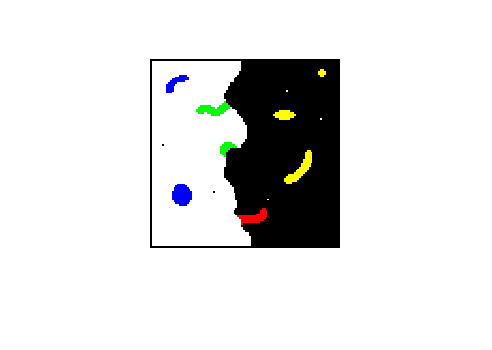
\includegraphics[width=5cm]{./Figs/binary_marks_clean_color_coded}}

\end{minipage}
\vspace{-0.5cm}
\caption{Binary salient regions detection.
Color coding: holes-blue, islands- yellow,
indentations - green, protrusions- red. }
\label{fig:binary_sal}
\end{figure}
%----------------------------------------------------------------------

\subsection{Data-driven binarization}
\label{ssec:binarize}
Any gray-scale image  $\I:~\mcD~\subset~\mathcal{Z}^2~\rightarrow ~\mcT $, where $\mcT=\{0,1,\ldots, t_{max}\}$ and $t_{max}~=~2^n-1~=~255$ is the maximum gray value encoded by $n~=~8$ bits, can be decomposed into cross-sections at
every possible level $t$:  $\I = \sum_{t \in \mcT}CS_t(\I)$. Obtaining a section at level $t$ is equivalent to thresholding the image at threshold $t$: $CS_t(\I)= 1.(\I>t) + 0.(\I<t)$ is a binary image. 
Three sets of connected components in $CS_t(\I)$ are defined: $\mcA_t$- {\em all}, $\mcL_t$- the {\em large} and $\mcV_t$- the {\em very large} CCs.  The size of each CC category is defined by$\Lambda_{\mcL}$ and $\Lambda_{\mcV}$ fraction of the image area $A_{\I}$. Let us denote the normalized number of elements in a set ($|\cdot|$) by $\Vert \cdot \Vert = |\cdot| / \max_{t \in \mcT}|\cdot|$.
Finding the optimal threshold $t_{opt}$ is then defined as:
\begin{equation*}
\vspace{-0.05cm}
t_{opt} = \argmax_{t \in \mcT}( w^{\mcA} \Vert \mcA_t \Vert + w^{\mcL} \Vert \mcL_t \Vert + w^{\mcV} \Vert \mcV_t \Vert ),
\vspace{-0.05cm}
\end{equation*}
where $w^{\cdot}$ are the weights per set of CCs.  

The standard Otsu thresholding does not select a single stable $CS$, while choosing $t_{opt}$ ensures stable number of regions across transformations (see Figs.~\ref{fig:binary_hist} and \ref{fig:leuven_bin} for lighting).
%------------------------------------------------------------------------
%\vspace{-0.8cm}
\begin{figure}[htb]

\begin{minipage}[b]{0.49\linewidth}
  \centering
  \centerline{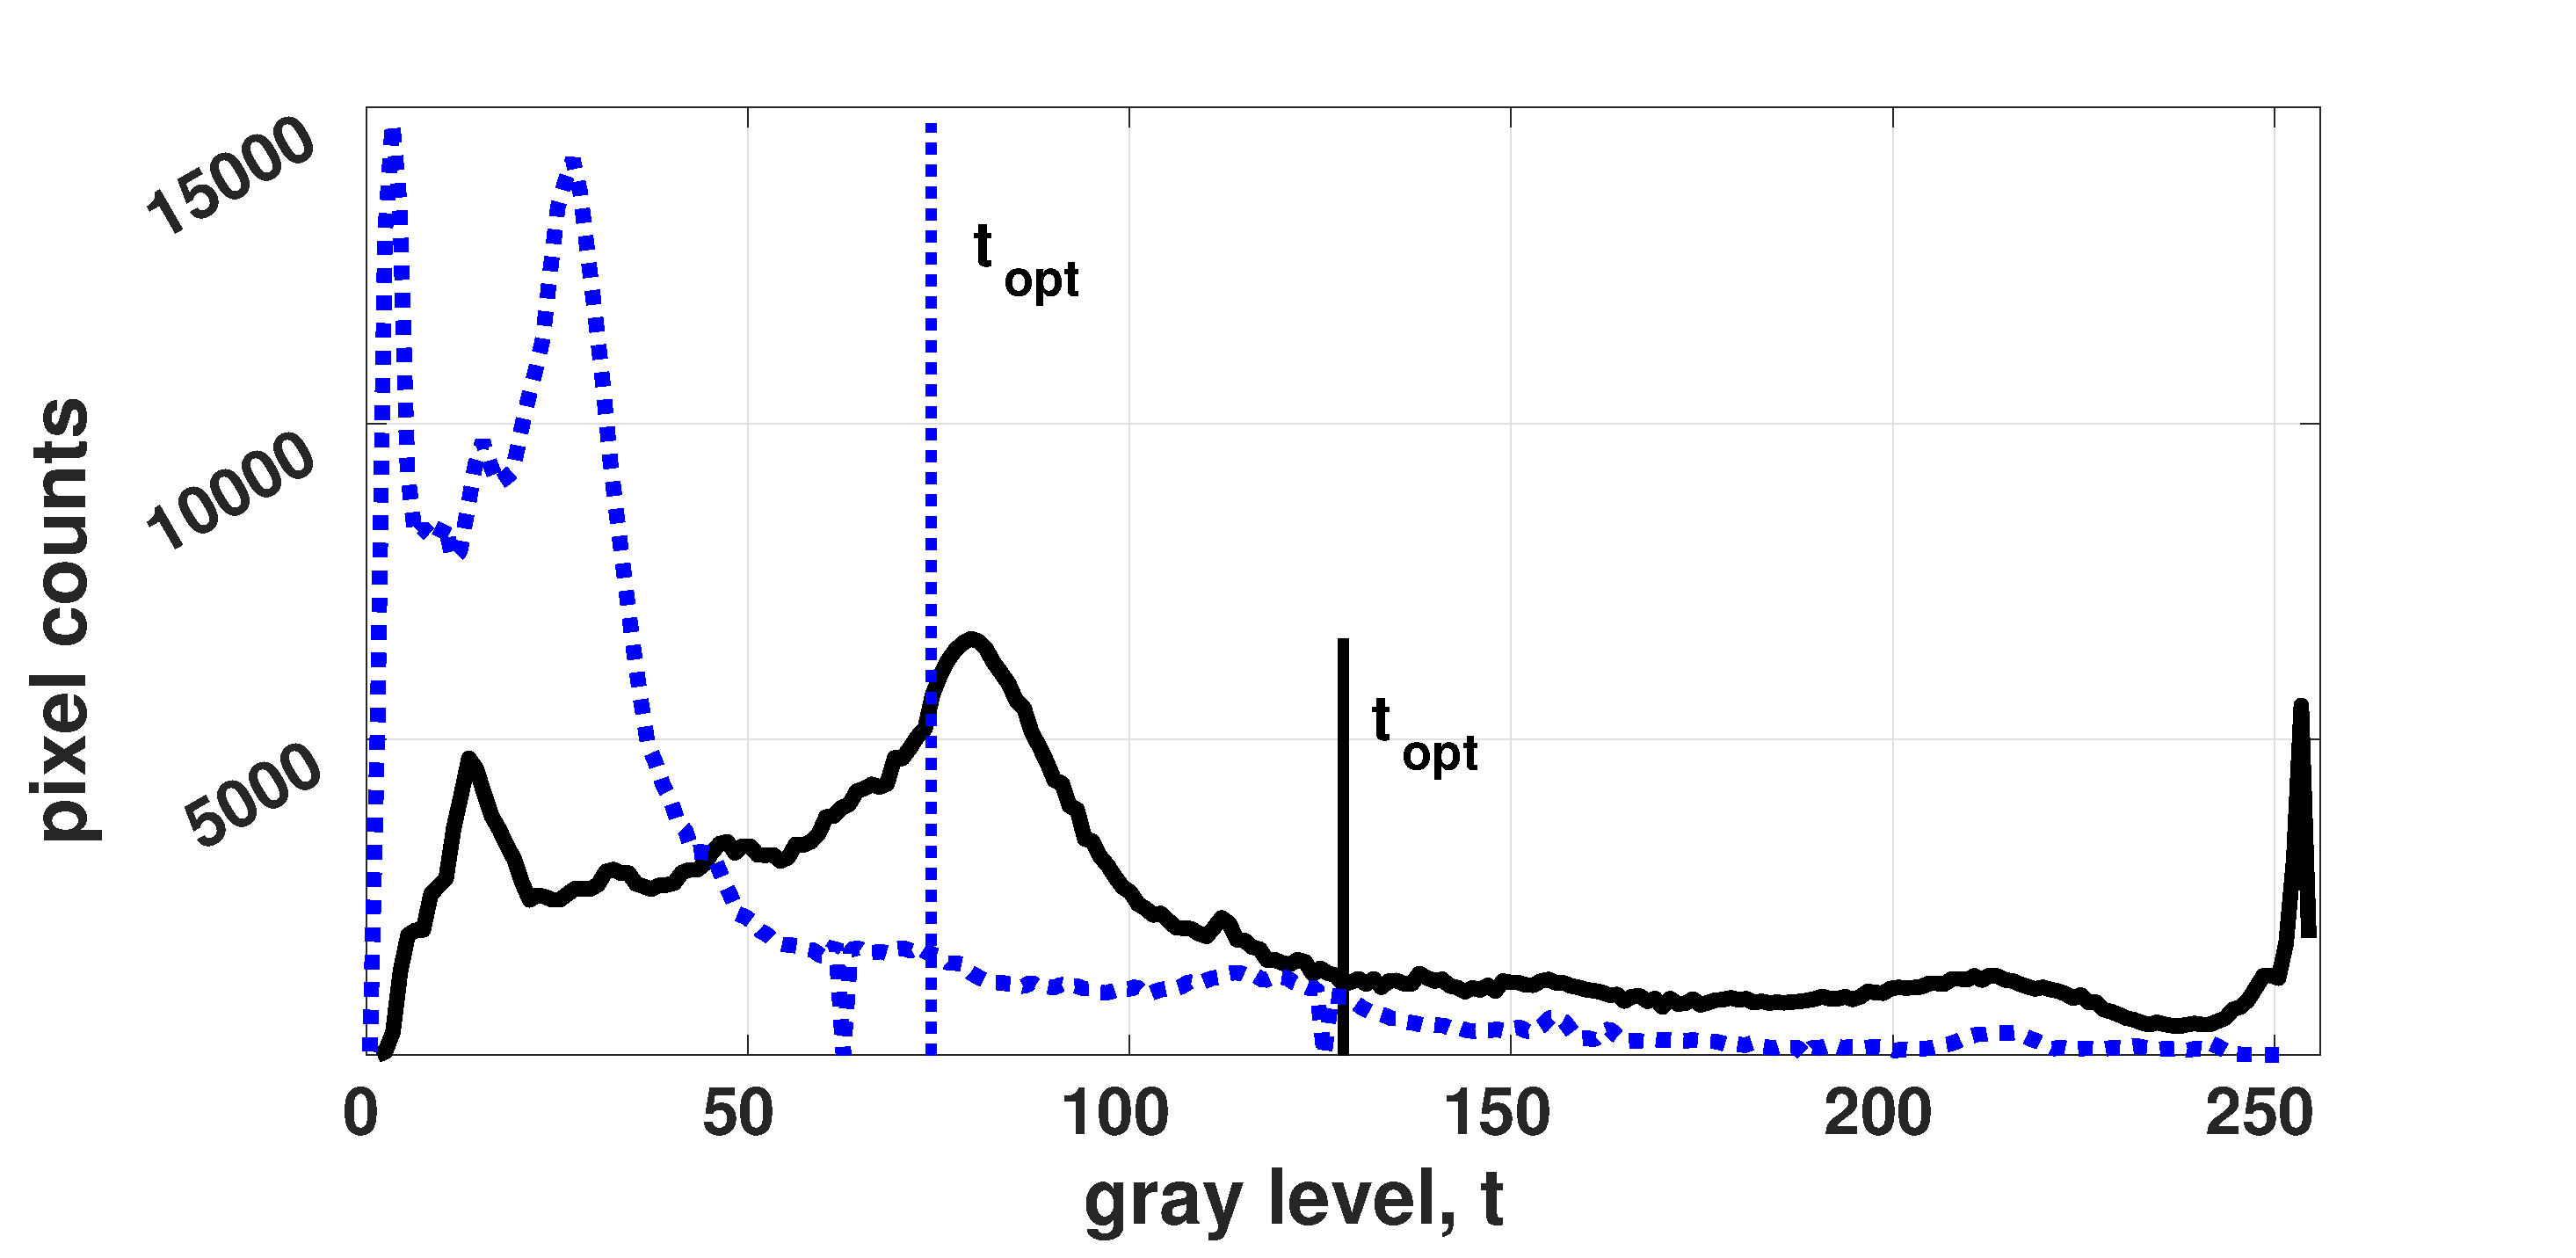
\includegraphics[width=4.65cm]{./Figs/hist_otsu_leuven_1_4}}
  \centerline{(a) Otsu}\medskip
\end{minipage}
\hfill
%\vspace{-0.5cm}
\begin{minipage}[b]{0.49\linewidth}
  \centering
  \centerline{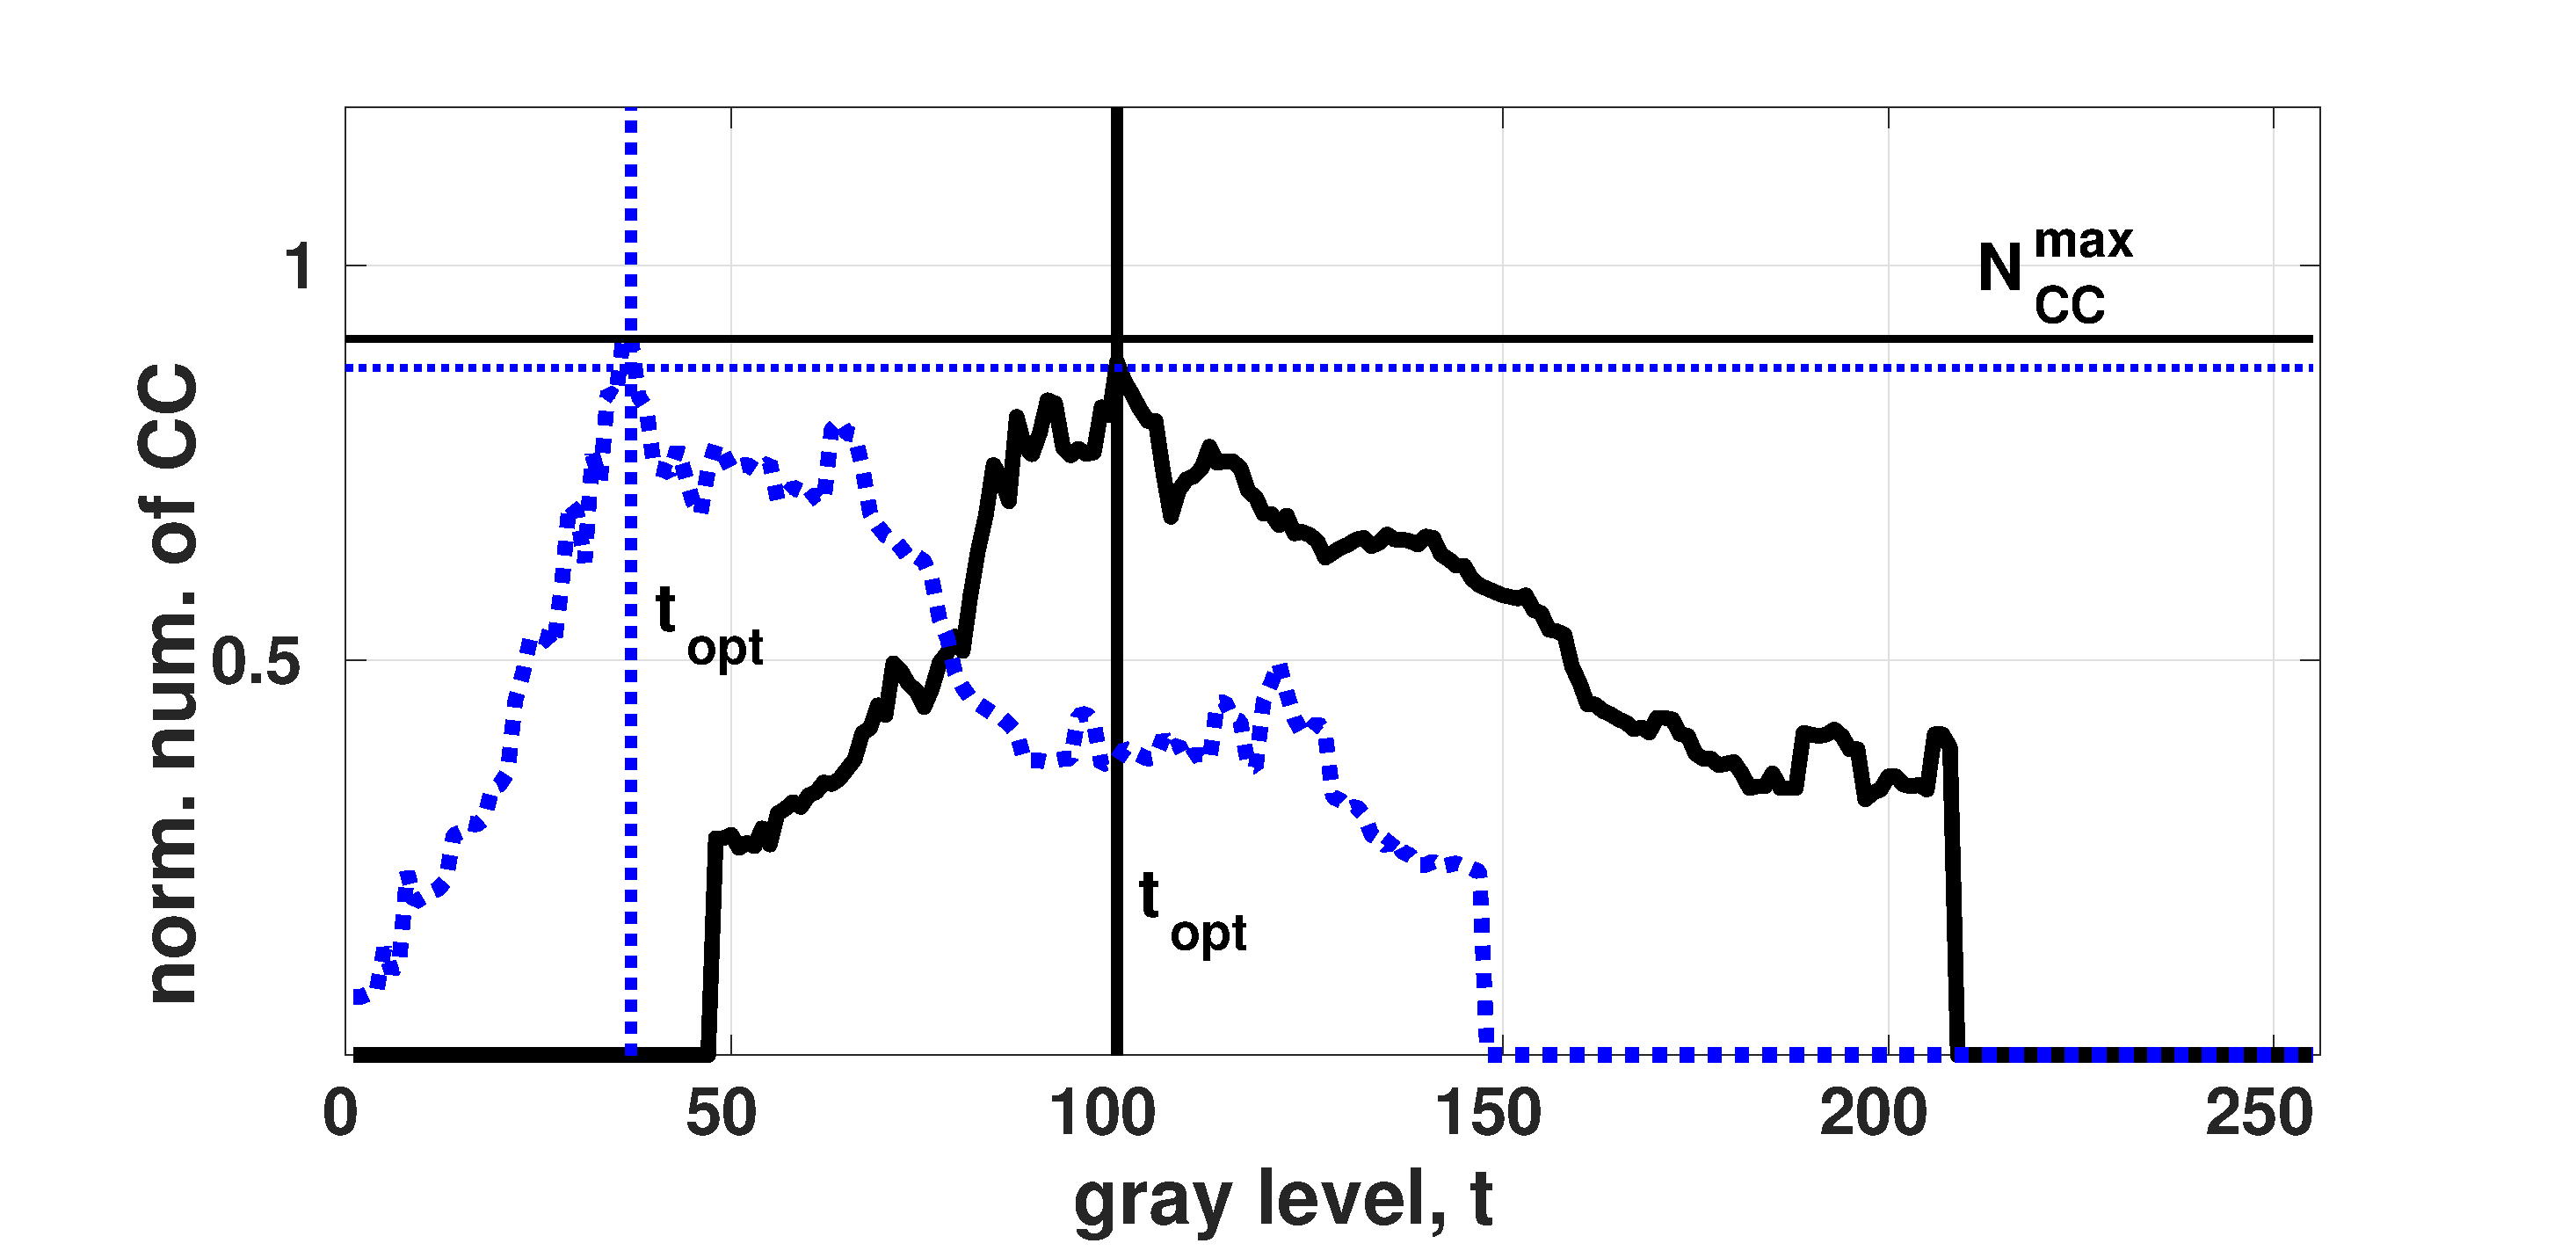
\includegraphics[width=4.8cm]{./Figs/hist_numcc_leuven_1_4}}
\centerline{(b) Max number CC}\medskip
\end{minipage}
\hfill
\vspace{-0.5cm}
\caption{Finding the optimal threshold for two images from the 'Leuven' sequence 
(Oxford dataset, lighting): the base image- solid black line, the forth image - dotted blue line.}
\label{fig:binary_hist}
%
\end{figure}
%------------------------------------------------------------------------
%\vspace{-0.5cm}

\begin{figure}[htb]

\begin{minipage}[b]{.3\linewidth}
  \centering
  \centerline{\includegraphics[width=2.8cm]{./Figs/leuven1}}
%  \vspace{1.5cm}
%   \centerline{(a)}\medskip
\end{minipage}
\hfill
\begin{minipage}[b]{0.3\linewidth}
  \centering
  \centerline{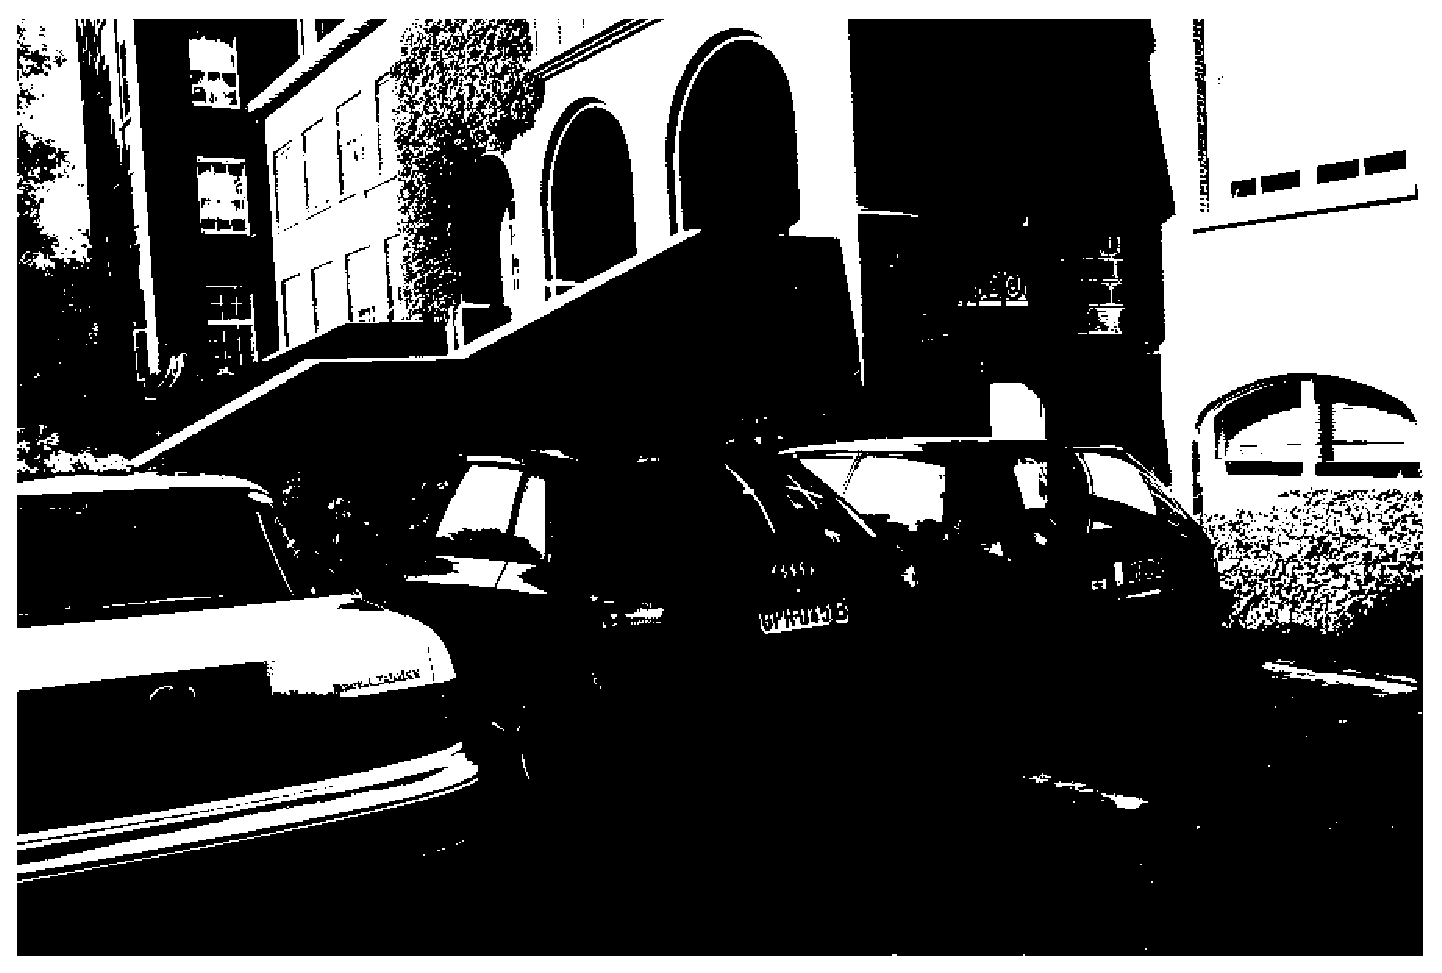
\includegraphics[width=2.7cm]{./Figs/leuven1_otsu}}
%  \vspace{1.5cm}
  % \centerline{(b)}\medskip
\end{minipage}
\hfill
\begin{minipage}[b]{0.3\linewidth}
  \centering
  \centerline{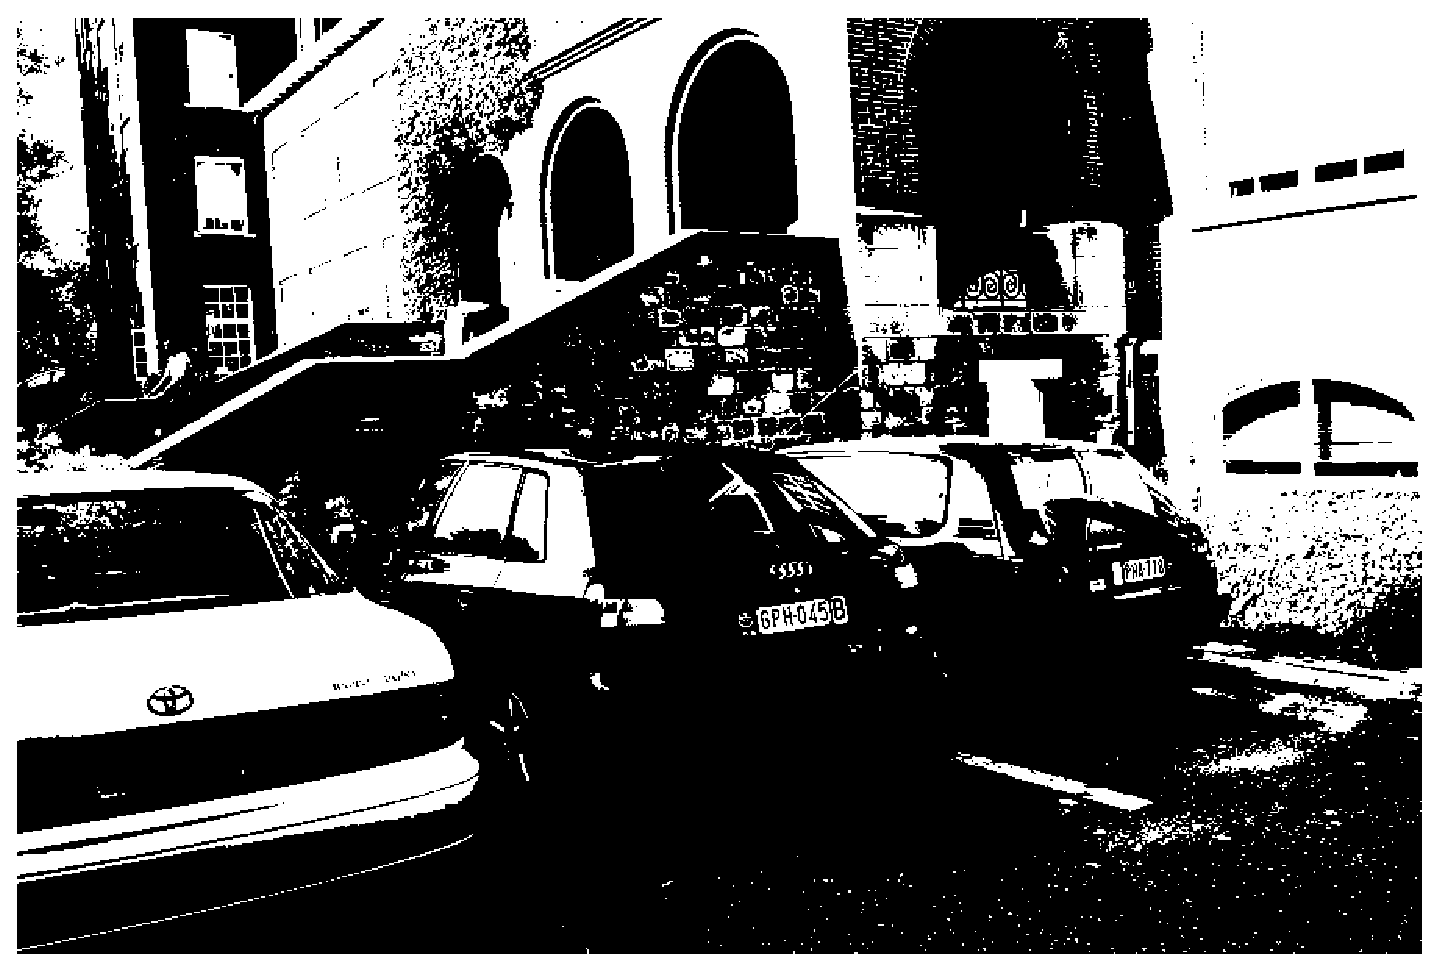
\includegraphics[width=2.7cm]{./Figs/leuven1_numcc}}
%  \vspace{1.5cm}
  % \centerline{(c)}\medskip
\end{minipage}

\begin{minipage}[b]{.3\linewidth}
  \centering
  \centerline{\includegraphics[width=2.7cm]{./Figs/leuven4}}
%  \vspace{1.5cm}
   \centerline{(a)}\medskip
\end{minipage}
\hfill
\begin{minipage}[b]{0.3\linewidth}
  \centering
  \centerline{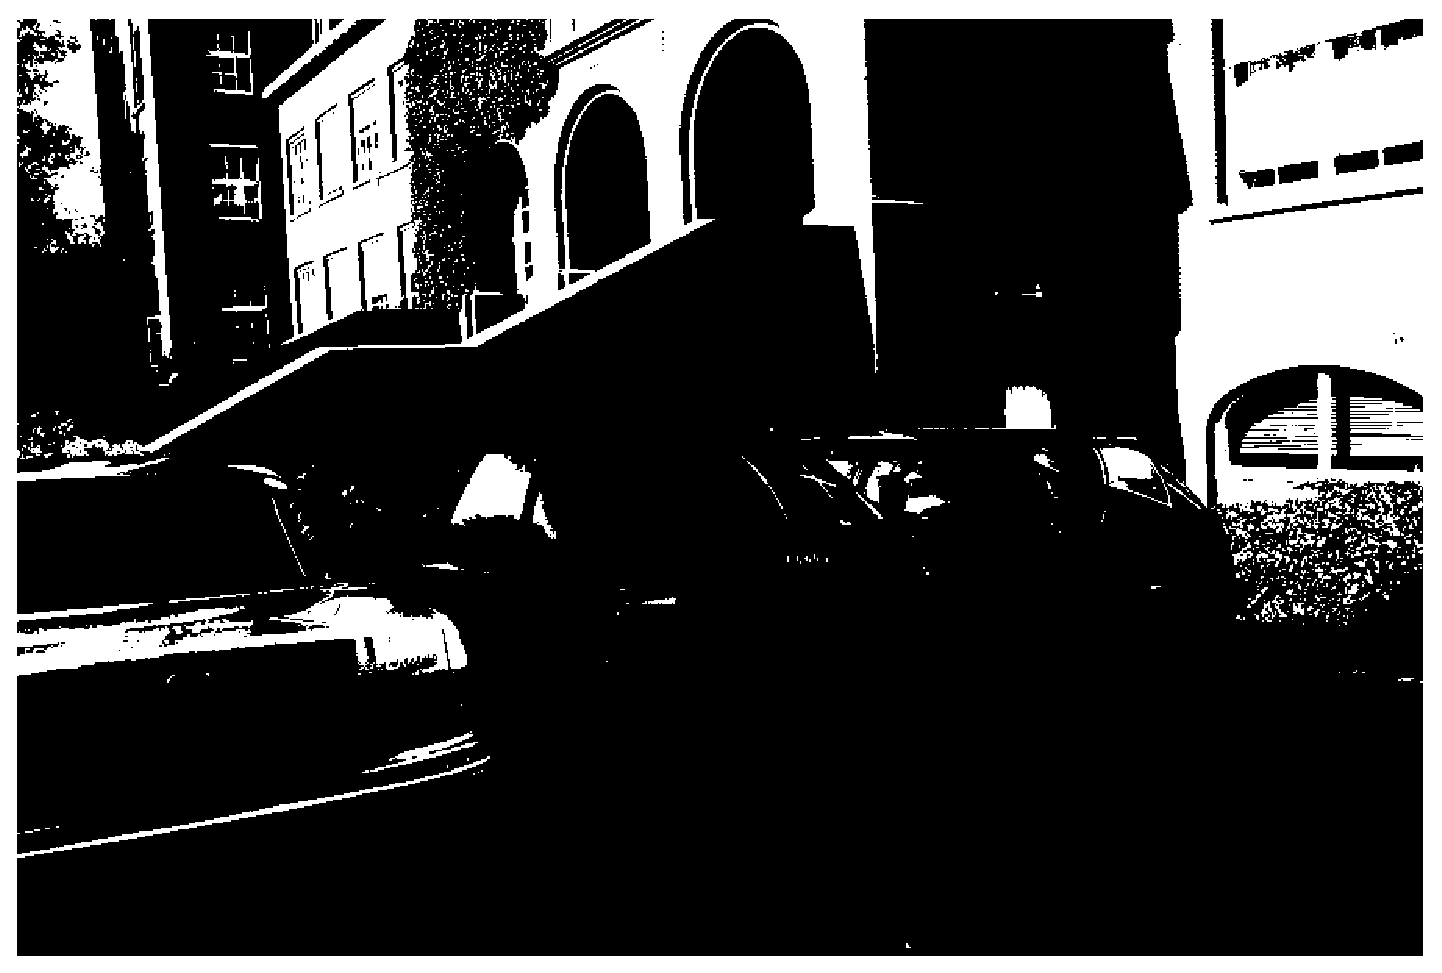
\includegraphics[width=2.7cm]{./Figs/leuven4_otsu}}
%  \vspace{1.5cm}
   \centerline{(b)}\medskip
\end{minipage}
\hfill
\begin{minipage}[b]{0.3\linewidth}
  \centering
  \centerline{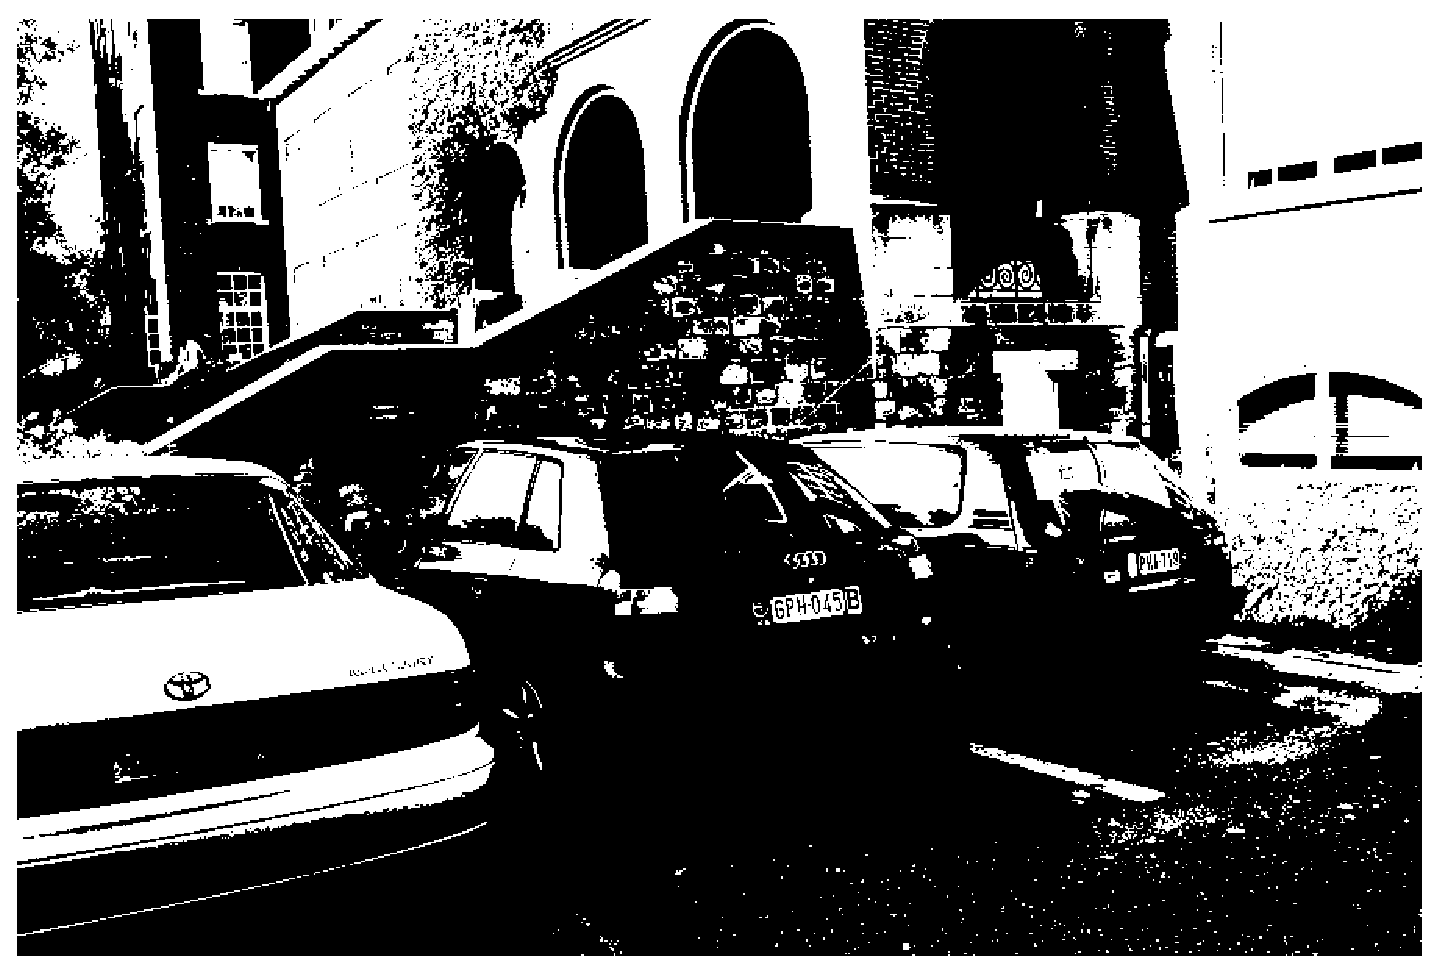
\includegraphics[width=2.7cm]{./Figs/leuven4_numcc}}
%  \vspace{1.5cm}
   \centerline{(c)}\medskip
\end{minipage}

 \vspace{-0.5cm}
\caption{Binarization of two images of the 'Leuven' sequence (lighting). Top row- base image, bottom row- forth image;   (a) gray scale; (b) Otsu binarization, (c) proposed binarization.}
\label{fig:leuven_bin}
%
\end{figure}
%------------------------------------------------------------------------

After the data-driven binarization, the DMSR detector finds the set of affine-covariant regions $\S$ from the single binary image $CS_{t_{opt}}$ as was described in Section \ref{ssec:binary} and \cite{RangMSSR06, RangHumpb06}. DMSR produces fewer non-overlapping and perceptually salient regions (visualized by their equivalent ellipses, not exact shapes) compared to MSER (see Figures~\ref{fig:det_graffiti} and \ref{fig:wood}).

\section{Performance  Evaluation}
\label{sec:perf}
{\em performance evaluation here...}
%------------------------------------------------------------------------
\begin{figure}[htb]

\begin{minipage}[b]{.49\linewidth}
  \centering
  \centerline{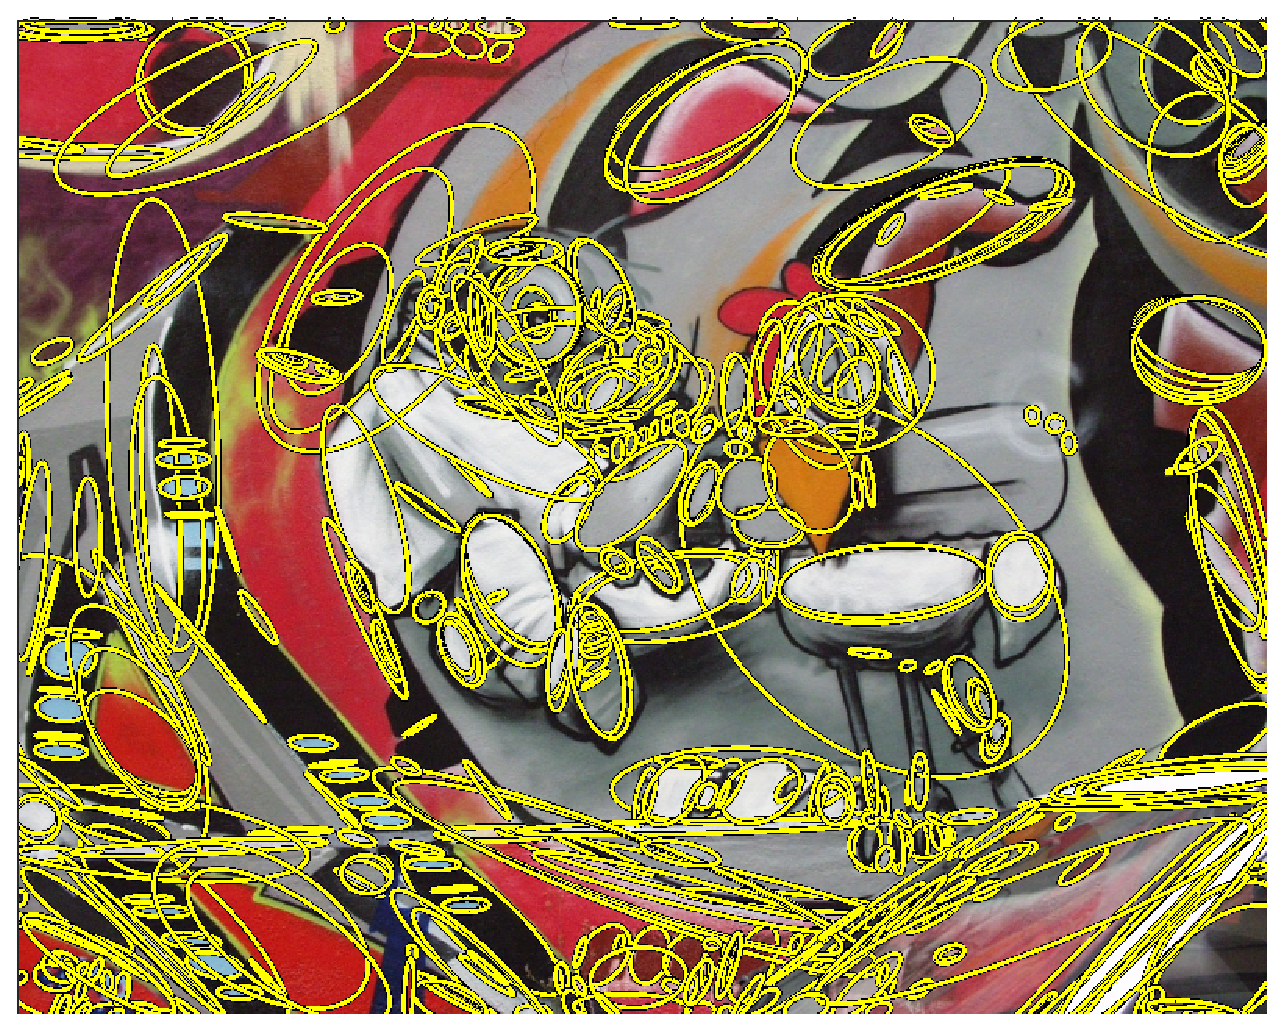
\includegraphics[width=4.0cm]{./Figs/mserGraffiti1}}
 % \vspace{0.2cm}
 % \centerline{(a) MSER}\medskip
\end{minipage}
\hfill
\begin{minipage}[b]{0.49\linewidth}
  \centering
  \centerline{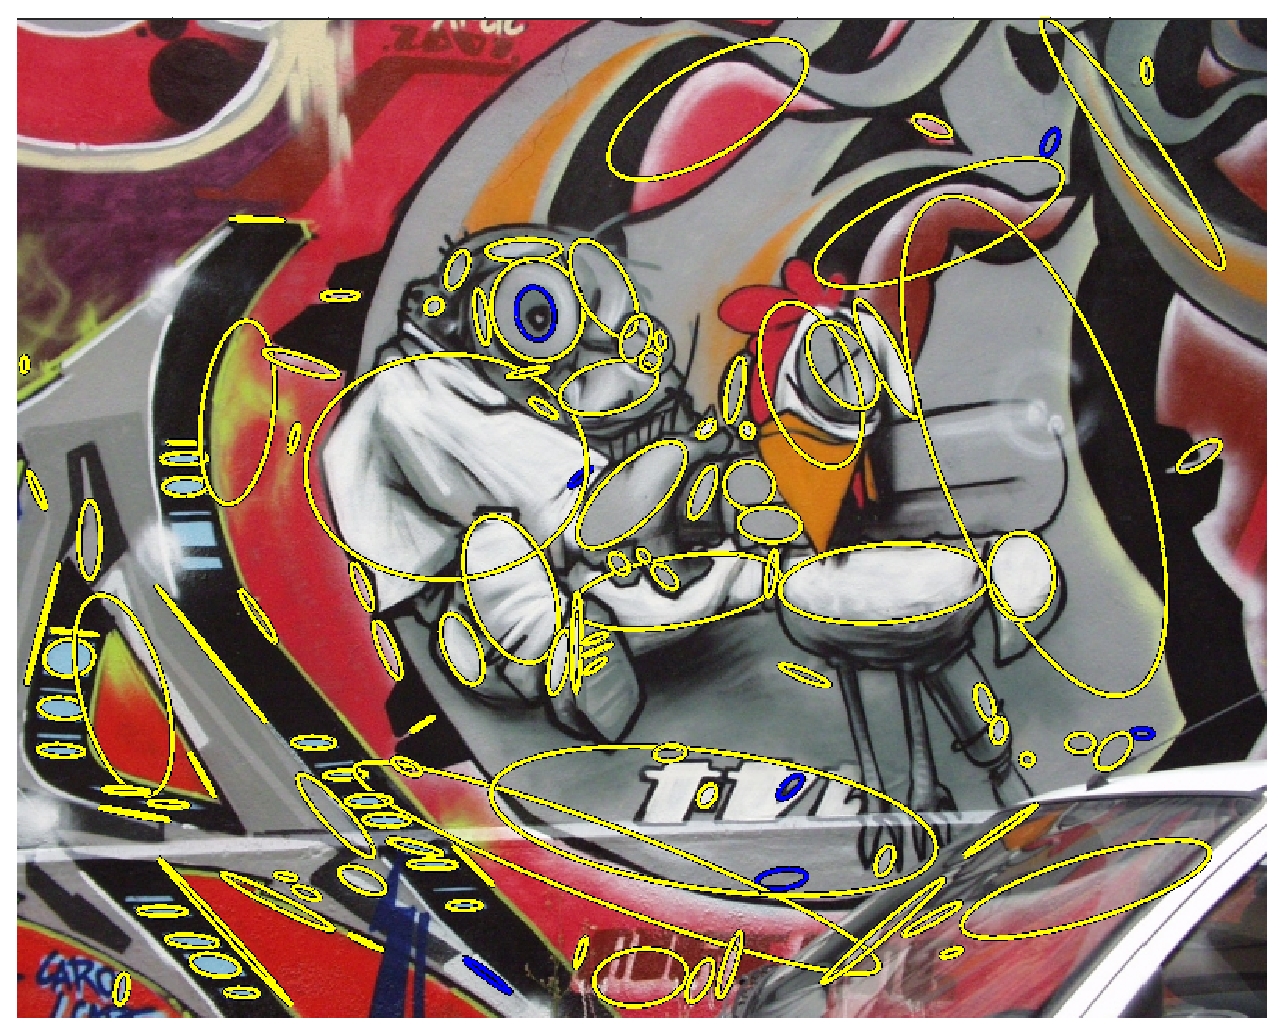
\includegraphics[width=4.0cm]{./Figs/dmsrGraffiti1}}
 % \vspace{0.2cm}
 % \centerline{(b) DMSR}\medskip
\end{minipage}
\vspace{-0.25cm}
\caption{Region detectors on the base image of the 'Graffiti' sequence, Oxford dataset. Left: MSER, right: DMSR}
\label{fig:det_graffiti}
%
\end{figure}
%------------------------------------------------------------------------
\begin{figure}[htb]

\begin{minipage}[b]{.49\linewidth}
  \centering
  \centerline{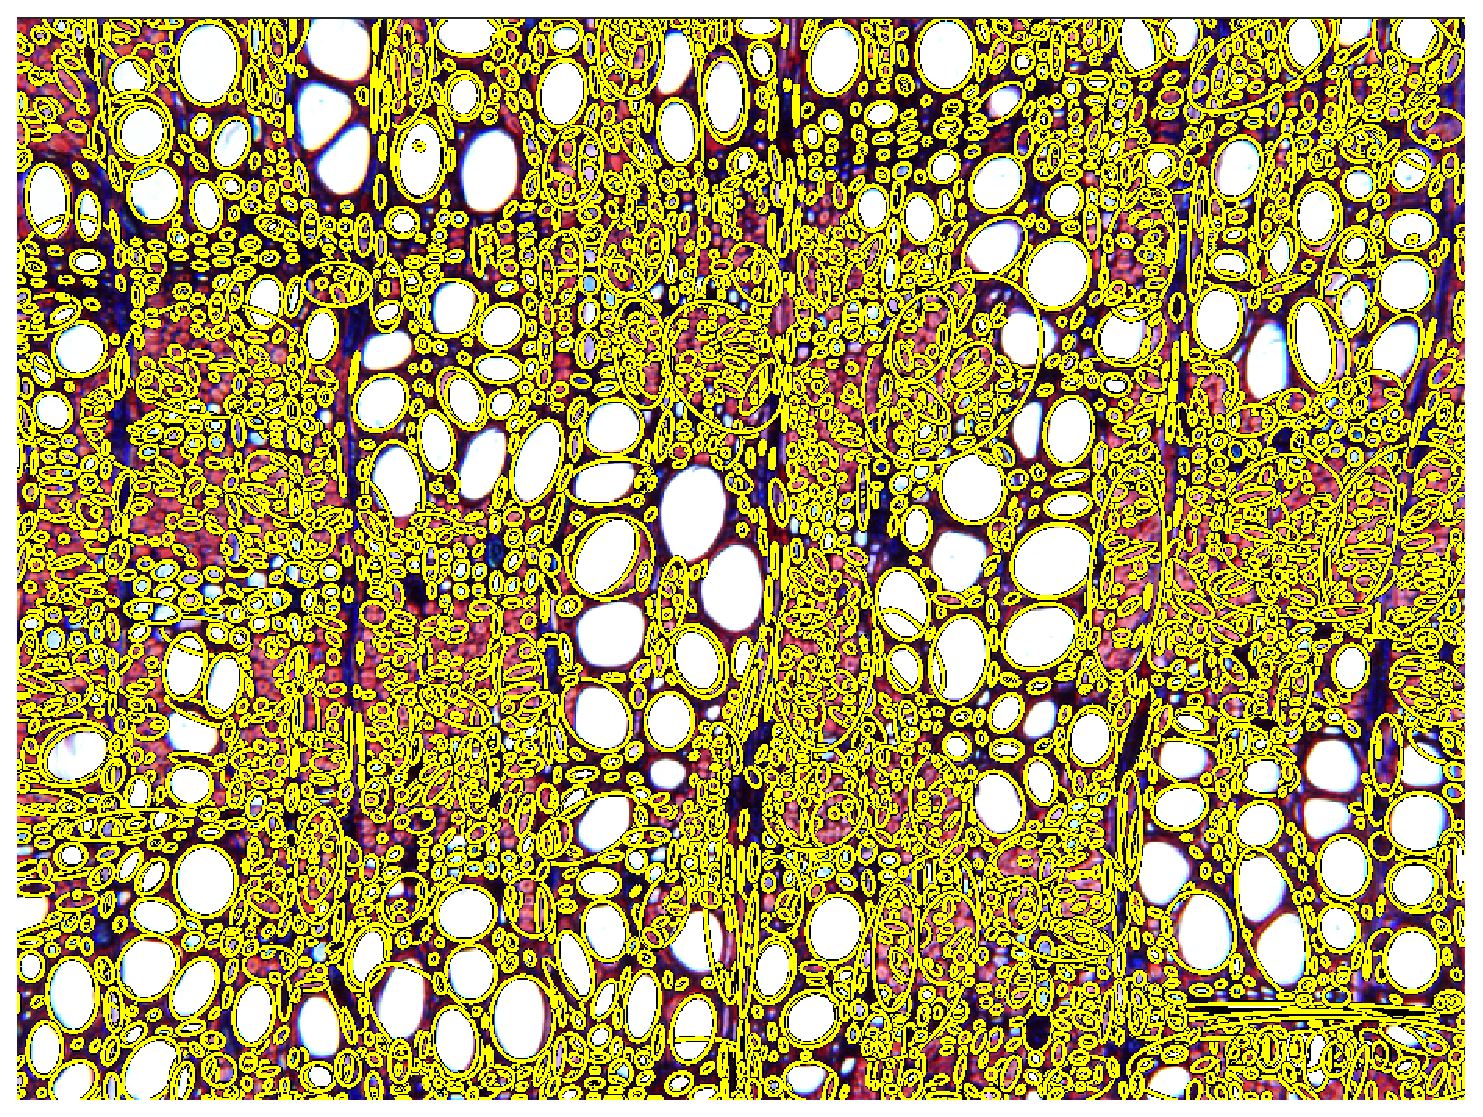
\includegraphics[width=4.0cm]{./Figs/mserWood}}
 % \vspace{0.2cm}
 % \centerline{(a) MSER}\medskip
\end{minipage}
\hfill
\begin{minipage}[b]{0.49\linewidth}
  \centering
  \centerline{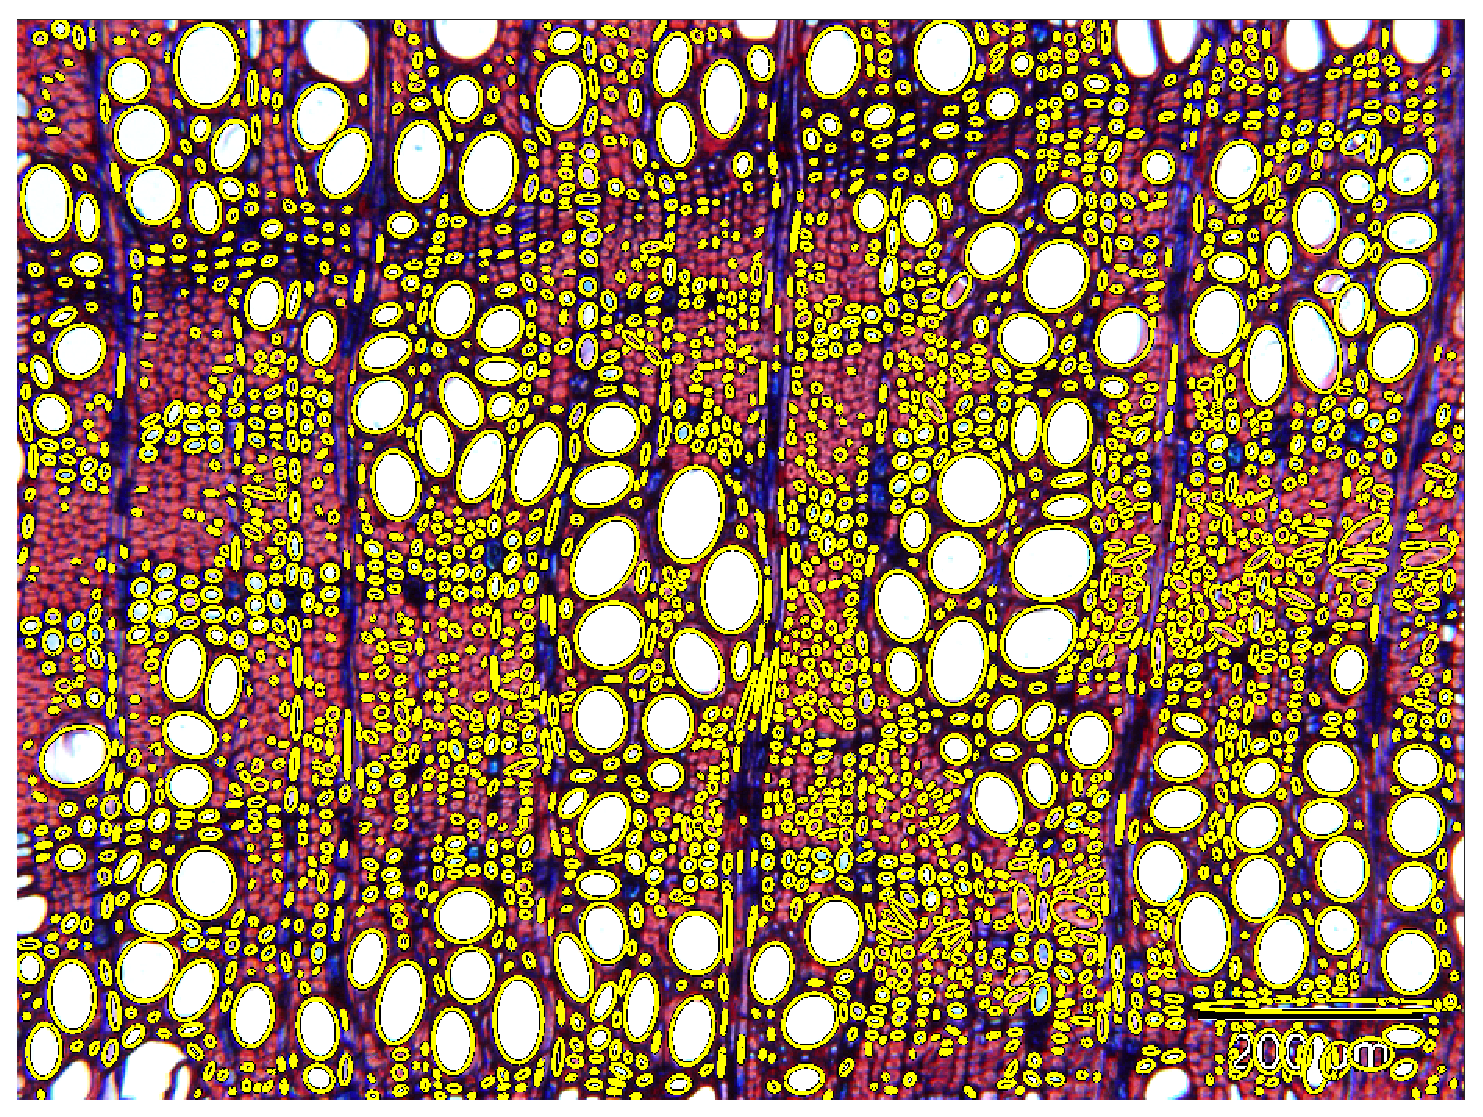
\includegraphics[width=4.0cm]{./Figs/dmsrWood}}
 % \vspace{0.2cm}
 % \centerline{(b) DMSR}\medskip
\end{minipage}
%\vspace{-0.25cm}
\caption{Salient region detectors on microscopy wood images. Left: MSER (every second region is shown), right: DMSR}
\label{fig:wood}
%
\end{figure}
%\vspace{-0.5cm}


% To start a new column (but not a new page) and help balance the last-page
% column length use \vfill\pagebreak.
% -------------------------------------------------------------------------
%\vfill
%\pagebreak


%\section{REFERENCES}
%\label{sec:ref}


% References should be produced using the bibtex program from suitable
% BiBTeX files (here: strings, refs, manuals). The IEEEbib.bst bibliography
% style file from IEEE produces unsorted bibliography list.
% -------------------------------------------------------------------------
\bibliographystyle{IEEEbib}
\bibliography{icip2016}

\end{document}
